\chapter{Concept Bottleneck Pipeline}
\label{concept-bottleneck-pipeline}


% TODO: a introduction to this chapter is useful
% Need to talk about what concept is here

% Things I need to include for Vikranth
%   precision values
%   concepts -> prediction MLP (both old and new)
%   maybe text classification


% Talk about Vikranth's work
\section{Inherited Work}
\label{inherited-work}

The work on the concept-bottleneck pipeline has not been done from scratch.

This chapter itself is a a continuation of the ideas proposed by Jeyakumar et al. in \emph{Automatic Concept Extraction for Concept Bottleneck-based Video Classification} \cite{RefWorks:RefID:16-2021automatic}, the paper which failed to meet the acceptance threshold for the \href{https://iclr.cc/}{ICLR 2022} conference. 

The main contribution the paper makes is the Concept Discovery and Extraction Module (CoDEx), a module which automatically uses video explanations to extract text concepts. \\
The authors shown that using the concepts extracted by CoDEx as a part of the concept bottleneck pipeline gives a comparable performance to a standard end-to-end model. 

\begin{figure}[h]
\caption{Schematic representation of the original concept bottleneck pipeline. The input in this case is an image but other types of input are also possible.}
\vspace{5pt}
\centering
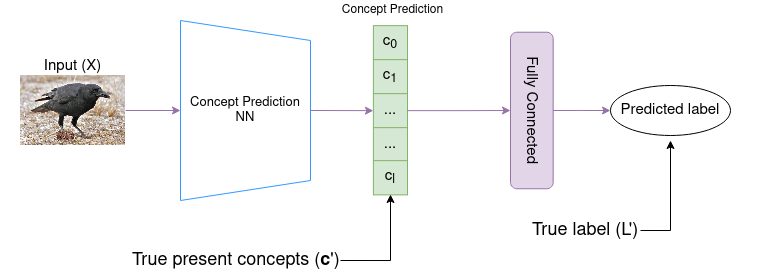
\includegraphics[width=\textwidth]{concept-bottleneck-pipeline/original-concept-bottleneck-model.png}
\label{original-concept-bottleneck}
\end{figure}

The idea from this project was inspired by the \emph{Concept Bottleneck Paper} \cite{RefWorks:RefID:35-koh2020concept}.
This paper shows that a neural network pipeline first predicting a set of relevant human-defined concepts, which are then used to predict the final label has a similar performance as an end-to-end network. 
A visualisation of a concept bottleneck pipeline can be seen in \ref{original-concept-bottleneck}.

Jeyakumar et al. replace the set of human-crafted true present concept by the output of a CoDEx. 
In addition, to better understand the impact each of the concept have on the final prediction, they add an attention layer after the concept layer to determine the concepts have more impact for the final prediction.
From that layer, they extract the top three concepts with the highest attention score which they use as explanations for a particular label.


% The contributions of the \emph{Automatic Concept Extraction for Concept Bottleneck-based Video Classification} can be summarised by the following points:
% \begin{itemize}
%  \item Concept Discovery and Extraction Module (CoDEx) is proposed, a module which automatically uses video explanations to extract concepts.
 
%  \item Model has been evaluated to validate it obtains competitive performance with standard end-to-end models.
 
%  \item The concept-based architecture has been augmented with the attention mechanism, which enables verifying how important each concept is for a decision.
 
%  \item Two public datasets are constructed, MLB-V2E and MSR-V2E. Both combine crowd-sourced explanations with short video sequences. The difference is that the MSR-V2E focuses mainly on general videos while MLB-V2E is baseball-related.
% \end{itemize}

The CoDEx is a vital element of the project.
The presented Concept Discovery and Extraction Module in the paper consists of 6 stages: cleaning, extraction, grouping, completion, pruning, and vectorisation. \\
The cleaning stage removes videos/explanations which are corrupted. \\
The extraction step uses a constituency parser and a rule-based approach to determine whether a part of the sentence  should be included as a candidate concept. 
The rules which the constituency parser uses to extract concepts are shown in the following table.

\begin{center}
\begin{tabular}{ |p{2cm}|p{12cm}|  }
 \hline
 \multicolumn{2}{|c|}{Rules determining whether a candidate concept should be included or excluded} \\
 \hline
 rule name & rule \\
 \hline
 Inclusion 1 & noun/pronoun → auxillary (optional) → particle (optional) → verb (optional) \\
 Inclusion 2 & noun/pronoun → auxiliary whose lemma is 'be' → any token \\
 Exclusion & subordinating conjunction \\
 
 \hline
 
\end{tabular}
\label{inclusion-exclusion-rules}
\end{center}

The completion stage looks up for concepts identified in some explanations while not other ones due to the behaviour of the constituency parser.
That stage is done by the substring lookup of existing concepts in all sentences where previous steps did not find that concept. \\
The grouping step attempts to group concepts with similar meanings using agglomerative clustering \cite{RefWorks:RefID:13-mullner2011modern}.  \\
The pruning stage attempts to keep highly informative concepts by picking the smallest concept subset such that the mutual information \cite{RefWorks:RefID:30-mackay2004information} between the label and a concept vector does not fall below a certain percentage $\gamma$.
This problem is not solved precisely, but rather concepts are inserted using a greedy approach until the mutual information between the label and the newly constructed vector is not below a percentage $\gamma$. The authors chose $\gamma = 0.9$ as an appropriate value. \\
The vectorisation constructs the N x K concept matrix, where K is the number of concepts and N is the number of data points. 
The cell (n, k) is one if the concept k occurs for the data point n, zero otherwise.

Jeyakumar et al. applied their idea to the MLB-V2E dataset, a baseball video dataset, resulting in the concept bottleneck pipeline diagram shown in figure \ref{vikranth-concept-bottleneck}.

\begin{figure}[h]
\caption{Schematic representation of the concept bottleneck pipeline presented by Jeyakumar et al. (adapted from \cite{RefWorks:RefID:16-2021automatic})} 
\vspace{5pt}
\centering
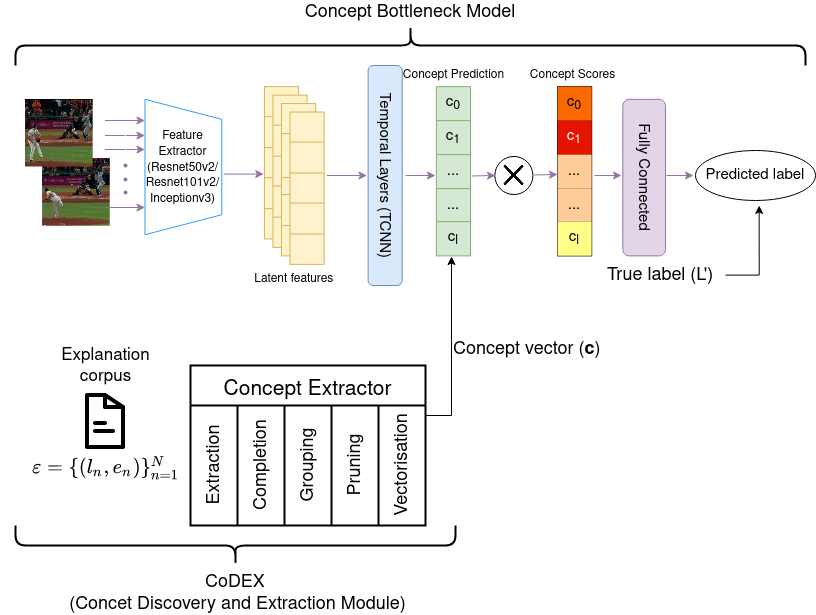
\includegraphics[width=\textwidth]{concept-bottleneck-pipeline/vikranth-concept-bottleneck.png}
\label{vikranth-concept-bottleneck}
\end{figure}

% Changes we made to the concept bottleneck pipeline
\section{Adaptions to the Concept Bottleneck Pipeline}

In this thesis, we adapted the CoDEx part of the concept bottleneck pipeline in order to improve the performance of the pipeline.

The extraction and the completion phase of the CoDEx have been removed from the pipeline.
The former used a rule based approach to extract concepts.
The latter finds all concepts discovered by the constituency parser in one sentence but not in another using substring matching.

The removed stages are quite simple and failed to account for a lot of information the video explanations conveyed.

To replace them extraction and completion we included \textbf{atomisation}, \textbf{generalisation} and \textbf{simple pruning} stage. \\
The first two stages (tasks) are explained in a great detail in chapter \ref{solving-nlp-tasks-logically}.
The \textbf{atomisation} stage splits provided sentences into one or more atomic sentences. 
Recall that the atomic sentences are sentences which cannot be decomposed into multiple valid sentences.
% INSERT ref to chapter 4
This procedure is done by using hand-crafted interpretable rule which is presented in the section \ref{solving-atomisation-task} along with the thought process for choosing the final solution.

The \textbf{generalisation} stage should extract all concept sentences from an atomic one. 
% INSERT refernce Sentence type definitions
As explained in the section \ref{sentence-type-definitions}, the concept sentence is a syntactically correct sentence that is obtained by modifying the syntax tree of a sentence.
To extract the concept sentences from an atomic sentence, we are using a solution learned by ILASP, with the learning procedure described in \ref{solving-generalisation-task}.

The \textbf{simple pruning} stage is the simplest out of any of the stages present. 
It removes the concept if it fails does not occur at least three times in the dataset.
If the concept fails to occur a few times in the entire dataset, it is likely that concept is only relevant to a specific video rather to the label. 
The generalisations of such a concept are more general and so occur more often.
This stage has almost no impact to the final set of concepts extracted because the \textbf{pruning} stage, which only keeps $K$ highly informative concepts, is very likely to eliminate low-frequency concepts.
Any dataset that we used had the identical final set of concepts with and without the simple pruning.
The benefit of this stages is that it reduces the number of irrelevant concepts before the \textbf{grouping} stage, greatly simplifying finding well-performing hyper-parameters required by that stage.

The diagram summarising the new concept bottleneck pipeline is shown in \ref{full-architecture-diagram}.

% TODO: fix X in picture, add boxes for the three parts, missing outlining X as attention module
\begin{figure}[h]
\caption{The full pipeline for the classification of MLB-V2E dataset using concept bottleneck model.} 
\centering
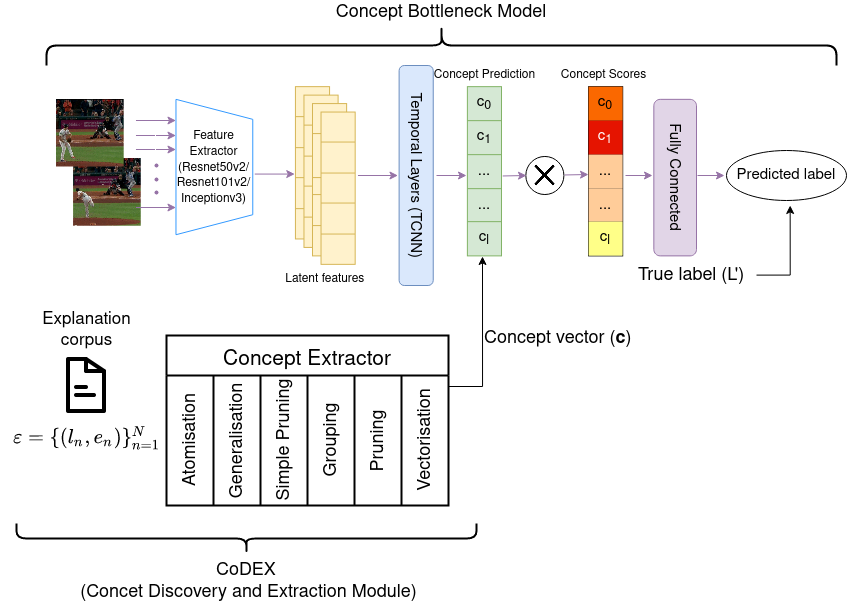
\includegraphics[width=\textwidth]{concept-bottleneck-pipeline/new-concept-bottleneck-pipeline.png}
\label{full-architecture-diagram}
\end{figure}

\section{Evaluation}

In this chapter, we will discuss how well does the newly presented CoDEx pipeline perform.
Any results produced will be compared with the previous iteration of the concept bottleneck pipeline and the uninterpretable end-to-end model, if applicable.
Each concept bottleneck model is trained using both joint and sequential models, unlike the \ref{inherited-work} which only uses the joint model.

% INSERT: Cite "do concept bottleneck models work as intended"
The difference between the two is that the joint optimises losses for both concepts and labels at the same time, which sometimes seems to overrule the nature of the concept bottleneck pipeline.
The sequential training model freezes the learned concept prediction layers so the final label has to be predicted from the concept predictions themselves.

% INSERT The caltech-ucsd birds-200-2011 dataset, Automated flower classification over a large number of classes
Also, we evaluate the concept bottleneck model on a new birds-flowers dataset, which combines randomly selected images from the CUB-200-2011 and 102 Category Flower Dataset along with their descriptions.
This evaluation inspects how well does the concept bottleneck pipeline translate to different domains.

Finally, we will critically analyse the strengths and limitations of the implemented method and suggest areas for future improvement.


\subsection{Measuring Cumulative MI}

% INSERT ref MacKay book; maybe insert Venn diagram from Wikipedia.  
Mutual Information $I(X;Y)$ \cite{RefWorks:RefID:30-mackay2004information} is defined as $I(X; Y) \equiv H(X) - H(X|Y)$. 
It estimates the average reduction in uncertainty about $x$ caused by understanding $y$'s value, or vice versa. 
It is the average quantity of information conveyed by $x$ regarding $y$.

In the context of this project, the discrete variable $Y$ is a set of label outcomes. A possible outcome is a number between 0 and 4 where each number represents an event which occurred.
The discrete variable $X$ represents a set of extracted concepts with size $k$, where $k$ is a parameter tested in this evaluation.

In addition, given that the cumulative MI is under consideration, the set of size $k$ should ideally contain $k$ \emph{maximally informative} concepts, i.e. those which combined will result in a highest mutual information score.
However, finding such a set is infeasible as the problem is combinatiorial \cite{RefWorks:RefID:16-2021automatic}, but we can get a highly informative set by greedily adding a single concept that improves MI the most. 

So, by measuring cumulative MI we can find out how good the extracted concepts are at describing the labels.

The results can be seen in \ref{cummulative-mi-graphs}.
It clearly shows that new concept extraction method greatly outperforms the old method.

\begin{figure}[h]
\caption{Cumulative MI graphs using old and new concept extraction pipeline}
\centering
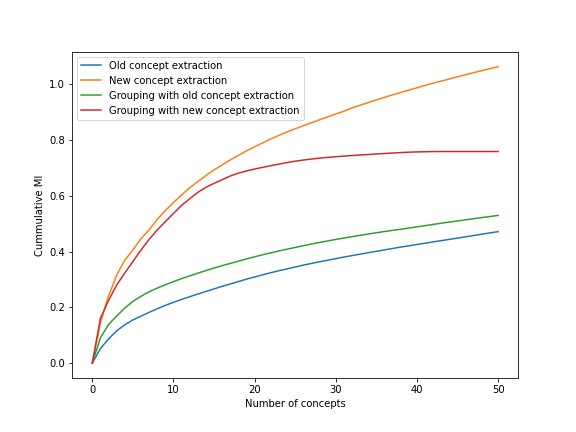
\includegraphics[width=\textwidth]{evaluation/Cummulative MI graphs.png}
\label{cummulative-mi-graphs}
\end{figure}

% TODO: talk about specific numbers

\subsection{Concept Prediction Performance}

A corollary of the higher informability of the concepts is a higher concept prediction accuracy.

Consider a classifier which would result in the highest possible accuracy for a dataset from binary vectors to labels.
Such a classifier with the maximum possible accuracy assigns the correct label to any non-conflicting binary vector and the most common label to any conflicting binary vector, a vector which might result in multiple different labels.

\begin{center}
\begin{tabular}{ |M{3 cm}||M{3cm}|M{3cm}|  }
 \hline
 \multicolumn{3}{|c|}{Maximum accuracy comparison} \\
 \hline
 \hline
  & Old Concept Extraction&New Concept extraction\\ 
 \hline
 Training dataset & 51.1\% & 78.6\% \\
 Test dataset & 47.7\% & 87.7\% \\
 \hline
\end{tabular}
\end{center}

Both training and test highest possible accuracies with the new concept extraction are much greater than the values achievable with the old procedure.

To validate whether we obtain similar results in practice, a multi-layer perceptron model from binary vectors to labels is trained with both old and new concept extraction.
% INSERT reference RoBERTa
As an estimate of how much information is lost through concept extraction, a RoBERTa transformer model is trained directly from unedited human-generated explanation.
% INSERT: figure comparing transformer MLP with 
The results are presented in figure X:


These experiments convince us that the performance of a concept bottleneck performance should improve.
They also suggest that there is still room for improvement for the concept extraction since there X\% accuracy improvement by using a model on the text itself.

\subsection{Performance of the Full Concept Bottleneck Pipeline}

The model performance is measured on the full concept bottleneck pipeline.
We measure the final accuracy of the models with identical architectures using new and old concept extraction. 
In addition, the quality of the concept prediction is also measured as it can help understand whether the concept bottleneck nature of the model is indeed considered.
The metric for measuring the concept prediction performance is F1, because for any datapoint, most concepts values are set to 0.
However, we do not want miss any of those concepts nor do we want the predictions to be incorrect because the predicted concept values should be crucial for final label prediction.
The final label prediction is measured using accuracy, as we want the predictions to be correct most of the time.
The predictive accuracies are also compared with an identical model that does not take concepts into account, the highest value the concept bottleneck models could achieve.

% TODO: insert model accuracy bar charts
The model accuracies are presented in figure X.

% TODO: analysis of the results

% TODO: Insert concept predictions bar charts
The concept prediction F1 scores are presented in figure X

% TODO: analysis of the resutls


\subsection{Explainability of the Labels}

The main reason we use the concept bottleneck pipeline is to allow interpretation of final labels using 


One of the main benefits of the concept bottleneck pipeline is its ability to explain

\subsection{Performance}

The two versions of the concept bottleneck pi
The concept bottleneck pipeline is compared against 

\subsection{Concept Bottleneck Pipeline Results}

In this subsection, we will see how does the new concept extraction perform when applied to the concept bottleneck pipeline.
The following models are compared in terms of explainability:
\begin{itemize}
    \item Concept Bottleneck Pipeline with old concepts.
    \item Concept Bottleneck Pipeline with new concepts.
\end{itemize}
In addition, two additional models are considered in performance measurements:
\begin{itemize}
    \item End-to-End model.
    \item MLB-Youtube model. 
\end{itemize}

% INSERT picture comparing architectures.
All three models intentionally have very similar architectures shown in X.
% INSERT hyper-parameter values
Moreover, the hyper-parameters are kept fixed at X across the runs for all models where we were in control of them


\subsubsection{Explainability}

% INSERT reference Mechanical Turk + original paper
As a part of \ref{inherited-work}, a Mechanical Turk study was preformed where the participants preferred the concept bottleneck results with attention in more than two-thirds of the cases.
Alternative choices were concept bottleneck results without attention, concepts of a random video from a different predicted class and a few randomly selected concepts from the set of most frequent concepts.


%  TODO: discuss with Luke and Ale about experiments
For this project a similar experiment was created. 
It additionally included a predicted set of concepts constructed with a new methods both before and after attention.

\subsubsection{Performance}


\subsubsection{Conclusion}

% New procedure is better

% \subsection{Old Evaluation Stuff}

% Despite this project being closely tied to the concept extraction from text, it will be researched and evaluated in the context of video classification.
% Utilising human-based explanations to improve the video classification outcome is quite a novel area since there are no projects that do precisely so.
% As such, there is no previous work the project will strive to do better than.\\

% However, for the approach proposed in the project to be considered a success, it must:

%  - Extract syntactic concept generalisations and create atomic sentences well. Both parts tasks will attempt to construct the solutions using machine learning/logic-based learning methods in a supervised setting. So, the methods proposed in this project should achieve small errors on relevant metrics.
 

%  - Do better than previous work which the supervisors have completed. As mentioned in the section \ref{completed-work}, this project continues on the paper currently under review for the ICLR 2022 conference. So, improving upon the method presented in the referenced work is imperative.
 
%  % INSERT reference
%  - Outperform all attempts made on the MLB-YouTube \cite{RefWorks:RefID:3-piergiovanni2018fine-grained} dataset. The dataset used, MLB-V2E \cite{RefWorks:RefID:16-2021automatic}, has taken its video clips from the segmented MLB-YouTube dataset and augmented it with crowd-sourced explanations. Given that the explanations were created by candidates familiar with baseball rules, they should contain all information needed to make correct classifications. 
%  In addition, Piergiovanni et al. \cite{RefWorks:RefID:3-piergiovanni2018fine-grained} argued that the MLB-YouTube is a challenging dataset to classify since the clips look similar. They are taken from the same camera angle, and the videos in different classes only differ by a fine-grained action.
%  So, with explanations, the overall task is much easier.
 
%  - Generalise to other datasets. The relevant metrics measuring error on concept generalisation and atomic sentence extraction should be similar when the method is applied to other datasets. It is possible to evaluate this project on the MSR-V2E \cite{RefWorks:RefID:16-2021automatic} dataset, which contains clips from everyday life and compare the performance with the MLB-V2E \cite{RefWorks:RefID:16-2021automatic} dataset.
 
%  - Be scalable. The performance of the concept extraction pipeline should not deteriorate when a bigger number of examples is given. To evaluate the scalability requirement, multiple models will be trained with a different number of examples and their performances compared.
 
%  - Be fast enough. This is a practical requirement. The machine learning model must not take too long to learn the needed representation. For example, it is unfeasible to have the model learn the concepts for more than 50 hours on the MLB-V2E dataset since one would need to evaluate it multiple times to facilitate the evaluation section of this project. Additionally, using the trained model on a test set example should be quick. The requirement mentioned will be measured by tracking how much time a model takes to complete a task.
 
%  - Enable adding MLB-V2E explanations for a video quickly. The concepts constructed by this project will be grammatically correct sentences. So, given that a concept can be detected in the video, it should be easy to create multiple sentences out of it. Further evaluation plans within this area will be considered later, depending on the time available for video explanation generation. Possibilities include having subjects judge whether the explanation is: incorrect both grammatically and logically, incorrect only grammatically, incorrect logically, good.\\
 
% The dataset with explanations is more costly and time-consuming to construct than the dataset without it.
% So, the final evaluation should also quantify this requirement (e.g. in terms of volunteer hours spent) while judging the feasibility and success of classification with crowd-sourced explanations.